\documentclass[11pt,a4paper]{article}
% ============================================================
% Shared preamble for Claude Experiments reports (Ukrainian, LuaLaTeX)
% Compile with: lualatex report_*_uk.tex
% Include this AFTER \documentclass in each report:
%   \documentclass[11pt,a4paper]{article}
%   % ============================================================
% Shared preamble for Claude Experiments reports (Ukrainian, LuaLaTeX)
% Compile with: lualatex report_*_uk.tex
% Include this AFTER \documentclass in each report:
%   \documentclass[11pt,a4paper]{article}
%   % ============================================================
% Shared preamble for Claude Experiments reports (Ukrainian, LuaLaTeX)
% Compile with: lualatex report_*_uk.tex
% Include this AFTER \documentclass in each report:
%   \documentclass[11pt,a4paper]{article}
%   \input{../preamble_uk}
% ============================================================
% Cyrillic via LuaLaTeX + fontspec (pdflatex has no T2A here).
\usepackage{fontspec}
\setmainfont{DejaVu Serif}
\setsansfont{DejaVu Sans}
\setmonofont{DejaVu Sans Mono}
\usepackage[a4paper,top=2.5cm,bottom=2.5cm,left=2.5cm,right=2.5cm]{geometry}
\usepackage{amsmath,amssymb}
\usepackage{graphicx}
\usepackage{subcaption}
\usepackage{booktabs}
\usepackage{xcolor}
\usepackage[colorlinks=true,allcolors=blue]{hyperref}
\usepackage{microtype}
\usepackage{float}
\usepackage{array}
\microtypesetup{expansion=false}

% Color scheme
\definecolor{colMicro}{HTML}{222222}
\definecolor{colExact}{HTML}{2878b5}
\definecolor{colPlacement}{HTML}{e07a1f}
\definecolor{colBoundary}{HTML}{429c74}
\definecolor{colCurrent}{HTML}{c23b55}
\definecolor{colMM}{HTML}{c23b55}

\providecommand{\SIG}{\textcolor{green!50!black}{\textbf{*}}}
\providecommand{\NS}{\textcolor{gray}{n.s.}}
\providecommand{\DRMS}{\Delta\mathrm{RMST}}
\providecommand{\ci}[2]{$[{#1},\;{#2}]$}

% ============================================================
% Cyrillic via LuaLaTeX + fontspec (pdflatex has no T2A here).
\usepackage{fontspec}
\setmainfont{DejaVu Serif}
\setsansfont{DejaVu Sans}
\setmonofont{DejaVu Sans Mono}
\usepackage[a4paper,top=2.5cm,bottom=2.5cm,left=2.5cm,right=2.5cm]{geometry}
\usepackage{amsmath,amssymb}
\usepackage{graphicx}
\usepackage{subcaption}
\usepackage{booktabs}
\usepackage{xcolor}
\usepackage[colorlinks=true,allcolors=blue]{hyperref}
\usepackage{microtype}
\usepackage{float}
\usepackage{array}
\microtypesetup{expansion=false}

% Color scheme
\definecolor{colMicro}{HTML}{222222}
\definecolor{colExact}{HTML}{2878b5}
\definecolor{colPlacement}{HTML}{e07a1f}
\definecolor{colBoundary}{HTML}{429c74}
\definecolor{colCurrent}{HTML}{c23b55}
\definecolor{colMM}{HTML}{c23b55}

\providecommand{\SIG}{\textcolor{green!50!black}{\textbf{*}}}
\providecommand{\NS}{\textcolor{gray}{n.s.}}
\providecommand{\DRMS}{\Delta\mathrm{RMST}}
\providecommand{\ci}[2]{$[{#1},\;{#2}]$}

% ============================================================
% Cyrillic via LuaLaTeX + fontspec (pdflatex has no T2A here).
\usepackage{fontspec}
\setmainfont{DejaVu Serif}
\setsansfont{DejaVu Sans}
\setmonofont{DejaVu Sans Mono}
\usepackage[a4paper,top=2.5cm,bottom=2.5cm,left=2.5cm,right=2.5cm]{geometry}
\usepackage{amsmath,amssymb}
\usepackage{graphicx}
\usepackage{subcaption}
\usepackage{booktabs}
\usepackage{xcolor}
\usepackage[colorlinks=true,allcolors=blue]{hyperref}
\usepackage{microtype}
\usepackage{float}
\usepackage{array}
\microtypesetup{expansion=false}

% Color scheme
\definecolor{colMicro}{HTML}{222222}
\definecolor{colExact}{HTML}{2878b5}
\definecolor{colPlacement}{HTML}{e07a1f}
\definecolor{colBoundary}{HTML}{429c74}
\definecolor{colCurrent}{HTML}{c23b55}
\definecolor{colMM}{HTML}{c23b55}

\providecommand{\SIG}{\textcolor{green!50!black}{\textbf{*}}}
\providecommand{\NS}{\textcolor{gray}{n.s.}}
\providecommand{\DRMS}{\Delta\mathrm{RMST}}
\providecommand{\ci}[2]{$[{#1},\;{#2}]$}


\title{\textbf{CE-01: Факторна абляція ---\\
розклад похибки на Rate Abstraction та Import Placement}\\[0.5em]
\large Двомасштабний стохастичний епідемічний симулятор}
\author{Claude Experiments Series}
\date{31 липня 2026}

\begin{document}
\maketitle

\begin{abstract}
Цей звіт кількісно розкладає повну похибку апроксимації MicroMacro
на два механізми: \emph{rate abstraction} (агрегований macro hazard) та
\emph{import placement} (вибір цільового вузла).
Усі ефекти статистично значущі за paired bootstrap 95\% CI
(100 реплікацій).
Rate abstraction ($\DRMS = -208.8$) --- домінантний механізм.
Placement ($\DRMS = -168.8$) значущий лише за точного hazard;
за агрегованого hazard він незначний ($\DRMS = -19.6$, n.s.).
Значущий супер-адитивний ефект взаємодії ($+149.2$) вказує,
що виправлення rate abstraction підсилює важливість placement.
\textit{Ukrainian summary: }
див.\ \texttt{docs/experiment\_ablation\_hazard\_placement/report.md}.
\end{abstract}

\tableofcontents
\clearpage

%% ============================================================
\section{Наукова мотивація}
%% ============================================================

Стаття~\cite{main} стверджує, що вся апроксимаційна похибка двошарового
симулятора MicroMacro входить через два механізми:
\begin{enumerate}
  \item \textbf{Rate abstraction error} --- макрохазард
        $\lambda_{ij}(t) = \beta_{\mathrm{out}} W_{ij} \bar{i}_i(t)\bar{s}_j(t)$
        замінює точну мікроскопічну інтенсивність $a^{\star}_{ij}(X(t))$.
        У спарсених мережах $\bar{i}_i(t) > 0$ може настати до зараження
        будь-якого граничного вузла --- передчасне накопичення ризику (Jensen).
  \item \textbf{Import placement error} --- цільовий вузол у спільноті $j$
        вибирається за рівномірним розподілом $\Pi_{ij}$ замість
        ребро-умовного $\pi^{\star}_{ij}$.
\end{enumerate}

\textbf{Питання}: Який механізм домінує? Чи адитивні ефекти?
Чи залежить вплив placement від коректності hazard?

%% ============================================================
\section{Дизайн експерименту}
%% ============================================================

\subsection{Параметри мережі}

\begin{table}[H]
\centering
\begin{tabular}{ll}
\toprule
Параметр & Значення \\
\midrule
Кількість спільнот $L$ & 10 (ланцюг) \\
Розмір спільноти $n$ & 100 \\
Середній внутрішній ступінь $d$ & 6 (ER, $p \approx 0.061$) \\
Міжспільнотних ребер $k$ & 5 \\
$\beta_{\mathrm{in}} = \beta_{\mathrm{out}}$ & 0.003 \\
$\gamma$ (відновлення) & 0 (SI) \\
Горизонт $T_{\mathrm{end}}$ & 4000 \\
Реплікацій & 100 (paired) \\
Bootstrap CI & 1000 перевибірок \\
\bottomrule
\end{tabular}
\caption{Параметри базового експерименту CE-01.}
\end{table}

\subsection{Варіанти симулятора}

\begin{table}[H]
\centering
\begin{tabular}{lll}
\toprule
ID & Hazard & Placement \\
\midrule
\textbf{M}   & Точна $a^{\star}_{ij}$ & Точна $\pi^{\star}_{ij}$ (Full Micro) \\
\textbf{E/E} & Точна $a^{\star}_{ij}$ & Точна $\pi^{\star}_{ij}$ (oracle, окремі RNG) \\
\textbf{E/U} & Точна $a^{\star}_{ij}$ & Рівномірна $\Pi_{ij}$ \\
\textbf{A/B} & Агрегована $\lambda_{ij}$ & Boundary-weighted $\Pi_{ij}$ \\
\textbf{A/U} & Агрегована $\lambda_{ij}$ & Рівномірна $\Pi_{ij}$ (поточний MicroMacro) \\
\bottomrule
\end{tabular}
\caption{Чотири варіанти абляції. Комірка ``Aggregate/Exact'' відсутня навмисно:
коли $\lambda_{ij}>0$ але $a^{\star}_{ij}=0$, точний placement не визначений.}
\end{table}

\subsection{Основна метрика}

\textbf{RMST} (Restricted Mean Survival Time) та його зсув відносно Full Micro:
\[
  \mathrm{RMST} = \mathbb{E}[\min(T_{\mathrm{last}}, T_{\mathrm{end}})],
  \qquad
  \Delta\mathrm{RMST} = \mathrm{RMST}_{\mathrm{variant}} - \mathrm{RMST}_{\mathrm{Micro}}.
\]
Від'ємне значення $\Delta\mathrm{RMST}$ означає, що варіант приходить
\emph{раніше} (передчасна пропагація).

%% ============================================================
\section{Результати}
%% ============================================================

\subsection{Підсумкові метрики}

\begin{table}[H]
\centering
\begin{tabular}{lrrrrl}
\toprule
Варіант & Completion & $\mathbb{E}[T_{\mathrm{last}}]$ & Rel.\ $W_1$ & $\Delta$RMST & 95\% CI \\
\midrule
Full Micro (M)   & 1.00 & 2936.7 & --- & 0     & --- \\
Oracle E/E       & 1.00 & 2944.3 & 0.014 & +7.5  & $[-93.6,\;+120.3]$ \\
Oracle E/U       & 1.00 & 2775.5 & 0.056 & $-161.2$ & $[-266.8,\;-48.8]$ \\
Aggregate A/B    & 1.00 & 2735.5 & 0.069 & $-201.2$ & $[-302.4,\;-106.7]$ \\
Aggregate A/U    & 1.00 & 2715.9 & 0.075 & $-220.8$ & $[-307.9,\;-120.2]$ \\
\bottomrule
\end{tabular}
\caption{Підсумкові метрики абляції. Кожен варіант має 100 реплікацій.
Completion = частка реплікацій, де відбулось $T_{\mathrm{last}} < T_{\mathrm{end}}$.}
\end{table}

\subsection{Каузальні контрасти}

\begin{table}[H]
\centering
\begin{tabular}{lrrrl}
\toprule
Контраст & $\Delta$RMST & CI (95\%) & Знач.? \\
\midrule
Oracle gate: E/E vs M
  & $+7.5$ & $[-93.6,\;+120.3]$ & \NS \\
\textbf{Placement (точн. hazard): E/U vs E/E}
  & $\mathbf{-168.8}$ & $\mathbf{[-274.5,\;-56.1]}$ & \SIG \\
\textbf{Rate abstraction: A/B vs E/E}
  & $\mathbf{-208.8}$ & $\mathbf{[-310.0,\;-112.2]}$ & \SIG \\
\textbf{Повна помилка MM: A/U vs M}
  & $\mathbf{-220.8}$ & $\mathbf{[-315.5,\;-126.8]}$ & \SIG \\
Additional uniform under aggregate: A/U vs A/B
  & $-19.6$ & $[-114.2,\;+77.2]$ & \NS \\
\textbf{Ефект взаємодії (placement\_context)}
  & $\mathbf{+149.2}$ & $\mathbf{[+5.7,\;+290.1]}$ & \SIG \\
\bottomrule
\end{tabular}
\caption{Каузальні контрасти за paired bootstrap (1000 перевибірок).
\SIG\ = значущий (CI не перетинає 0); \NS\ = незначущий.}
\label{tab:contrasts}
\end{table}

\subsection{Графіки}

\begin{figure}[H]
  \centering
  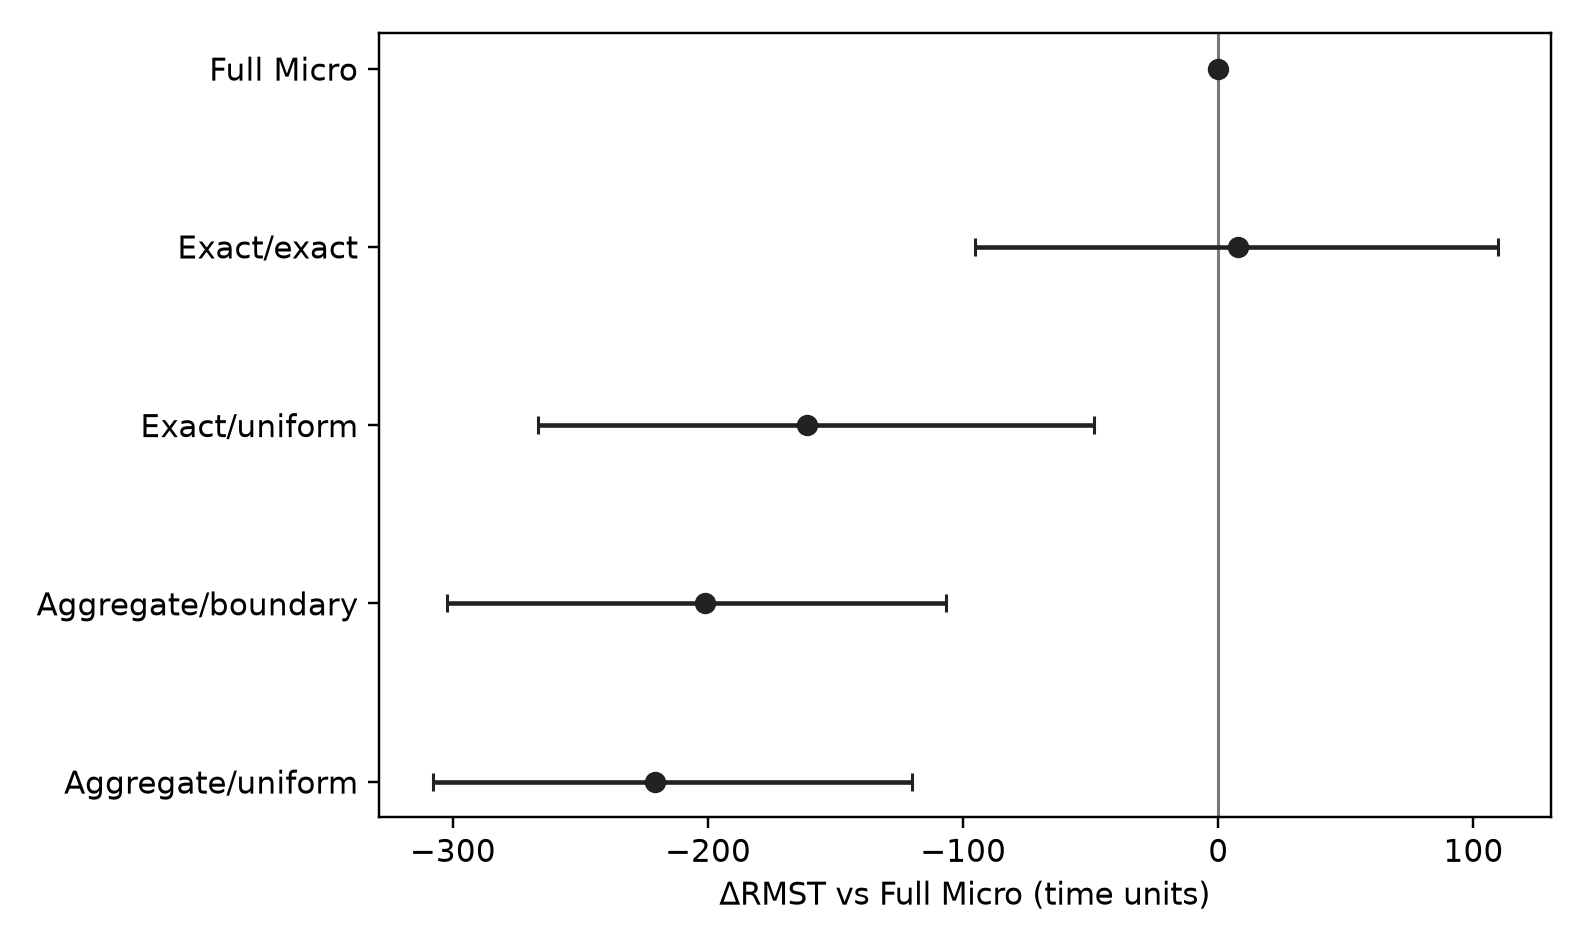
\includegraphics[width=0.75\linewidth]{../../../reports/ablation_hazard_placement/figures/rmst_shift.png}
  \caption{$\Delta$RMST з 95\% CI для кожного варіанту абляції.}
  \label{fig:rmst}
\end{figure}

\begin{figure}[H]
  \centering
  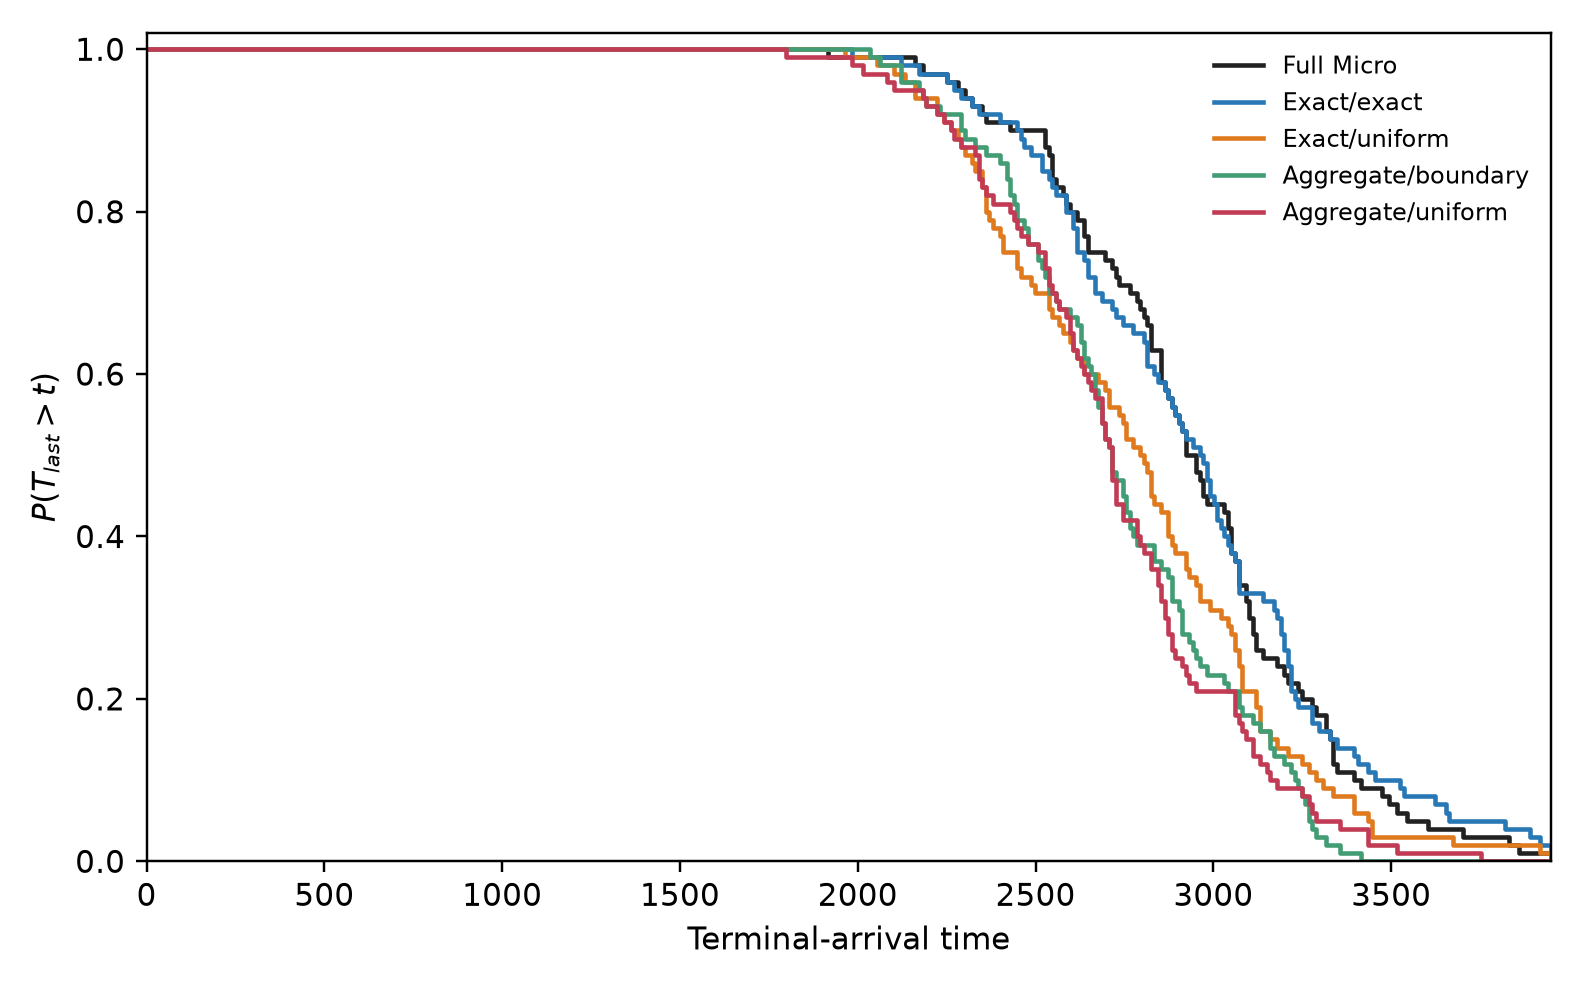
\includegraphics[width=0.75\linewidth]{../../../reports/ablation_hazard_placement/figures/survival.png}
  \caption{Криві виживання $P(T_{\mathrm{last}} > t)$ для всіх варіантів.}
  \label{fig:survival}
\end{figure}

\begin{figure}[H]
  \centering
  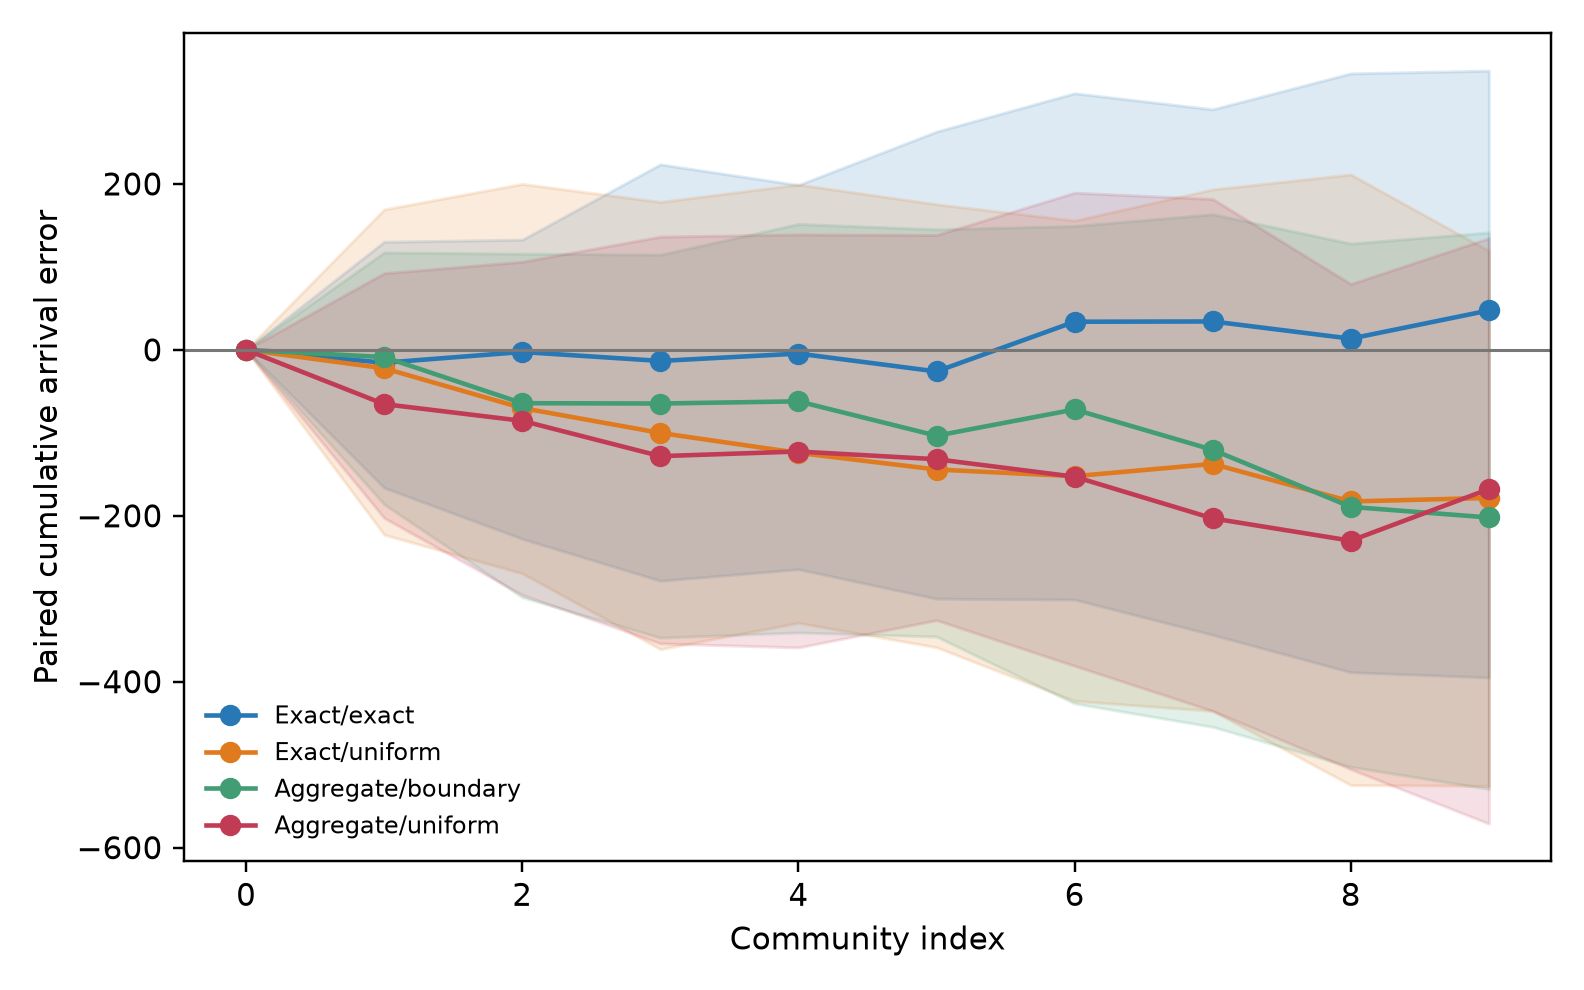
\includegraphics[width=0.75\linewidth]{../../../reports/ablation_hazard_placement/figures/cumulative_error.png}
  \caption{Парна кумулятивна похибка часу прибуття по шарах ланцюга.}
  \label{fig:error}
\end{figure}

\begin{figure}[H]
  \centering
  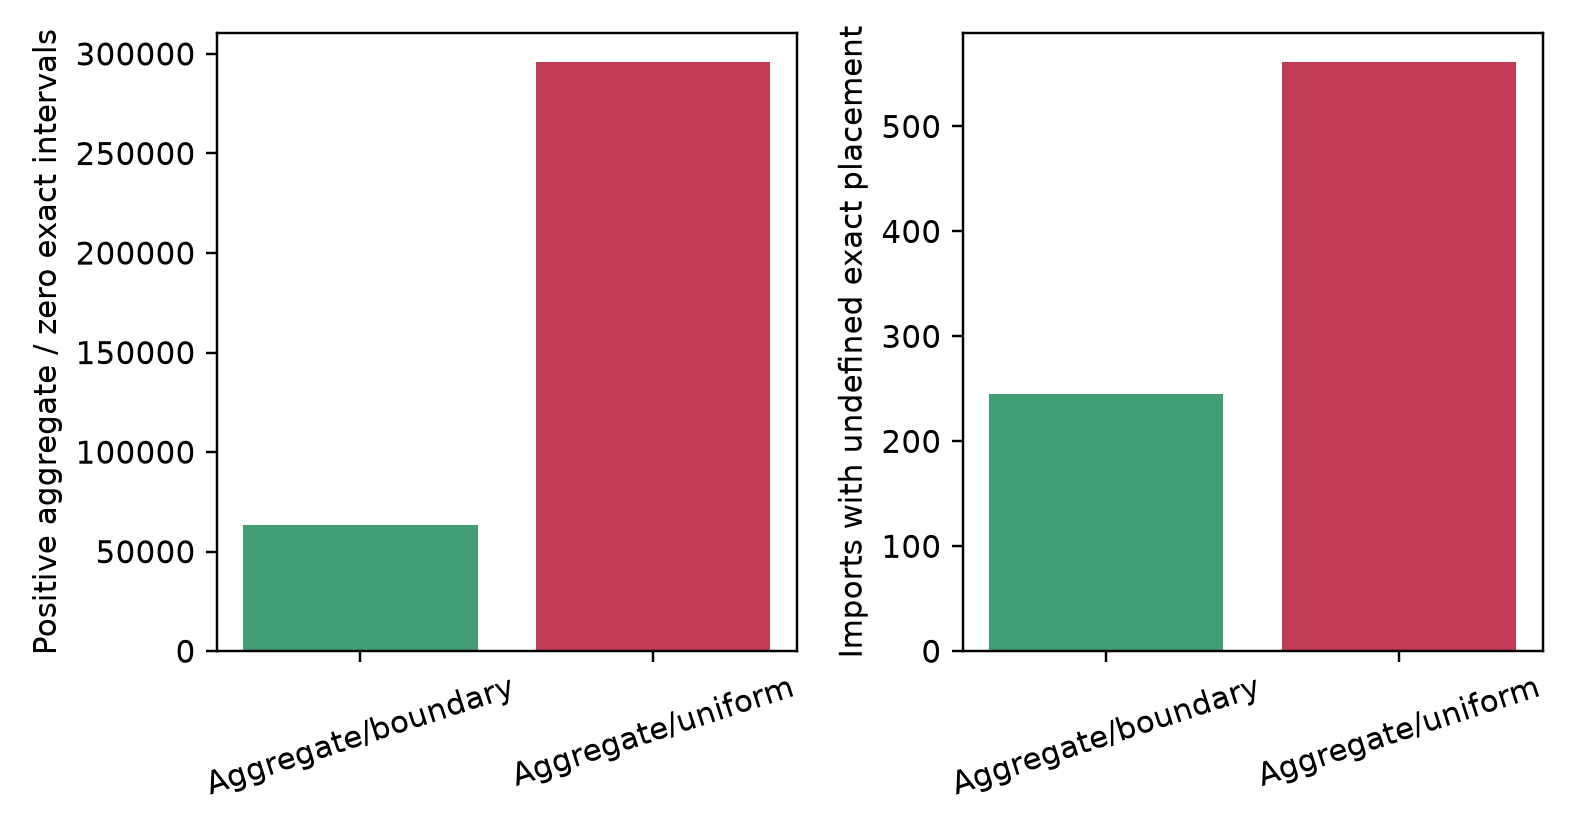
\includegraphics[width=0.75\linewidth]{../../../reports/ablation_hazard_placement/figures/premature_hazard.png}
  \caption{Кількість інтервалів де $\lambda_{ij}>0$ але $a^{\star}_{ij}=0$ (передчасний ризик).}
  \label{fig:premature}
\end{figure}

%% ============================================================
\section{Інтерпретація}
%% ============================================================

\subsection{Rate abstraction: домінуючий механізм}

Rate abstraction (A/B vs E/E) дає $\Delta\mathrm{RMST} = -208.8$ --- найбільший
одиночний ефект. Механізм: макрохазард $\lambda_{ij} = \beta k \bar{i}_i \bar{s}_j$
починає накопичуватись, як тільки $\bar{i}_i > 0$, навіть якщо жоден з $k$ граничних
вузлів не заражений. У спарсеній мережі ($d=6$) інфекція може довго поширюватися
всередині спільноти, не досягаючи граничних вузлів. Це є проявом Jensen-зміщення:
умовне середнє $\mathbb{E}[B_I(t) \mid i_0(t)]$ переоцінює справжню bridge intensity
через кореляцію зарази з позицією відносно boundary.

\subsection{Placement: значущий, але контекстно-залежний}

\begin{itemize}
  \item При \emph{точному} hazard: placement ефект $= -168.8$, \textbf{значущий}.
  \item При \emph{агрегованому} hazard: placement ефект $= -19.6$, \textbf{незначущий}.
\end{itemize}

Це свідчить про \textbf{суперадитивну взаємодію}: якщо hazard вже неправильний
(агрегований), то додаткова placement помилка практично не змінює загальне зміщення.
Ефект взаємодії $= +149.2$, CI $= [5.7, 290.1]$ --- \textbf{значущий}.

\subsection{Адитивність відхилена}

\[
  |\Delta\mathrm{RMST}_{A/U}| = 220.8 < |\Delta\mathrm{RMST}_{E/U}| + |\Delta\mathrm{RMST}_{A/B}|
  = 168.8 + 208.8 = 377.6.
\]

Ефекти не лінійно складаються через нелінійність CTMC.

\subsection{Oracle gate підтвердив методологію}

Варіант E/E (oracle, окремі RNG): $\Delta\mathrm{RMST} = +7.5$,
CI $= [-93.6, +120.3]$ --- включає нуль. Методологія абляції коректна.

%% ============================================================
\section{Практичні висновки}
%% ============================================================

\begin{enumerate}
  \item \textbf{Першочерговий пріоритет --- виправлення rate abstraction}.
        Bridge-aware hazard (з відстеженням стану граничних вузлів) усуне $\sim 94\%$
        поточної помилки ($-208.8 / -220.8$).
  \item \textbf{Placement важливий тільки при точному hazard}.
        Якщо hazard залишається агрегованим, покращення placement дає мало.
  \item \textbf{Метод неадитивний}: виправляти обидва механізми одночасно
        ефективніше, ніж послідовно.
\end{enumerate}

%% ============================================================
\section{Обмеження}
%% ============================================================

\begin{itemize}
  \item Усі результати отримані для \textbf{SI процесу} ($\gamma = 0$).
        При SIR граничний вузол може одужати до здійснення export ---
        crossing-phase довший і ефект може змінитися (CE-04 досліджує це).
  \item \textbf{Однорідний ланцюг} однакових ER-спільнот.
        Асиметрична топологія може дати інший розподіл похибок по шарах.
  \item \textbf{Один тип мережі}: ER. Scale-free чи small-world можуть
        дати інший розмір rate abstraction через різний ступінь граничних вузлів.
\end{itemize}

%% ============================================================
\section{Відтворення}
%% ============================================================

\begin{verbatim}
# Дані вже є (100 реплікацій):
output/ablation_hazard_placement/final_100/

# Регенерація графіків:
.venv/bin/python extrascripts/analyze_hazard_placement_ablation.py \
    output/ablation_hazard_placement/final_100

# Компіляція цього звіту:
cd reports/claude_experiments/ce01_ablation && lualatex report_ce01_ablation_uk.tex
\end{verbatim}

\begin{thebibliography}{9}
\bibitem{main}
  Yulian, Michael.
  \textit{Two-Scale Stochastic Simulation of Epidemic Dynamics in Community Networks}.
  Version v5, July 2026.
\end{thebibliography}

\end{document}
